%%%%%%%%%%%%%%%%%%%%%%%%%%%%%%%%%%%%%%%%%%%%%%%%%%%%%%%%%%%%%%%%%%%%%%%%%%%%%%%
\documentclass[hyperref={pdfpagelabels=false},compress,table]{beamer} % 在Mac下无法编译
% \documentclass[compress,table]{beamer} % 在Mac下使用
% package for font
\usepackage{fontspec}
\defaultfontfeatures{Mapping=tex-text}  %%如果没有它,会有一些 tex 特殊字符无法正常使用,比如连字符。
\usepackage{xunicode,xltxtra}
\usepackage[BoldFont,SlantFont,CJKnumber,CJKchecksingle]{xeCJK}  % \CJKnumber{12345}: 一万二千三百四十五
\usepackage{CJKfntef}  %%实现对汉字加点、下划线等。
\usepackage{pifont}  % \ding{}
% package for math
\usepackage{amsfonts}

% package for graphics
\usepackage[americaninductors,europeanresistors]{circuitikz}
\usepackage{tikz}
\usetikzlibrary{plotmarks}  % placements=positioning
\usepackage{graphicx}  % \includegraphics[]{}
\usepackage{subfigure}  %%图形或表格并排排列
% package for table
\usepackage{colortbl,dcolumn}  %% 彩色表格
\usepackage{multirow}
\usepackage{multicol}
\usepackage{booktabs}
% package for code
\usepackage{fancyvrb}
\usepackage{listings}

% \usepackage{animate}
% \usepackage{movie15}

%%%%%
% setting for beamer
\usetheme{default} % Madrid(常用), Copenhagen, AnnArbor, boxes(白色), Frankfurt,Berkeley
\useoutertheme[subsection=true]{miniframes} % 使用Berkeley时注释本行
\usecolortheme{sidebartab}
\usefonttheme{serif}  %%英文使用衬线字体
% \setbeamertemplate{background canvas}[vertical
% shading][bottom=white,top=structure.fg!7] %%背景色,上25%的蓝,过渡到下白。
\setbeamertemplate{theorems}[numbered]
\setbeamertemplate{navigation symbols}{}  %% 去掉页面下方默认的导航条
\setbeamercovered{transparent}  %设置 beamer 覆盖效果

% 设置标题title背景色
% \setbeamercolor{title}{fg=black, bg=lightgray!60!white}
\setbeamercolor{title}{fg=white, bg=black!70!white}

% 设置每页小LOGO
\pgfdeclareimage[width=1cm]{ouc}{figures/static/ouc.pdf}
\logo{\pgfuseimage{ouc}{\vspace{-20pt}}}

% setting for font
%%\setCJKmainfont{Adobe Kaiti Std}
\setCJKmainfont{SimSun} 
%% \setCJKmainfont{FangSong_GB2312} 
%% \setmainfont{Apple Garamond}  %%苹果字体没有SmallCaps
\setCJKmainfont{SimSun} 
%FUNNY%\setCJKmainfont{DFPShaoNvW5-GB}  %%华康少女文字W5(P)
%FUNNY%\setCJKmainfont{FZJingLeiS-R-GB}  %%方正静蕾体
%FUNNY%\setmainfont{Purisa}
%\setsansfont[Mapping=tex-text]{Adobe Song Std}
     %如果装了Adobe Acrobat,可在font.conf中配置Adobe字体的路径以使用其中文字体。
     %也可直接使用系统中的中文字体如SimSun、SimHei、微软雅黑等。
     %原来beamer用的字体是sans family;注意Mapping的大小写,不能写错。
     %设置字体时也可以直接用字体名,以下三种方式等同:
     %\setromanfont[BoldFont={黑体}]{宋体}
     %\setromanfont[BoldFont={SimHei}]{SimSun}
     %\setromanfont[BoldFont={"[simhei.ttf]"}]{"[simsun.ttc]"}
% setting for graphics
\graphicspath{{figures/}}  %%图片路径
\renewcommand\figurename{图}

% setting for pdf
\hypersetup{% pdfpagemode=FullScreen,%
            pdfauthor={Xiaodong Wang},%
            pdftitle={Title},%
            CJKbookmarks=true,%
            bookmarksnumbered=true,%
            bookmarksopen=false,%
            plainpages=false,%
            colorlinks=true,%
            citecolor=green,%
            filecolor=magenta,%
            linkcolor=blue,%red(default)
            urlcolor=cyan}

% setting for fontspec
\XeTeXlinebreaklocale "zh"  %%表示用中文的断行
\XeTeXlinebreakskip = 0pt plus 1pt minus 0.1pt  %%多一点调整的空间
%%%%%

% font setting by xeCJK
\setCJKfamilyfont{NSimSun}{NSimSun}
\newcommand{\song}{\CJKfamily{NSimSun}}
%%%\setCJKfamilyfont{AdobeSongStd}{Adobe Song Std}
%%%\newcommand{\AdobeSong}{\CJKfamily{AdobeSongStd}}
\setCJKfamilyfont{FangSong}{FangSong_GB2312}
\newcommand{\fang}{\CJKfamily{FangSong}}
%%%\setCJKfamilyfont{AdobeFangsongStd}{Adobe Fangsong Std}
%%%\newcommand{\AdobeFang}{\CJKfamily{AdobeFangsongStd}}
\setCJKfamilyfont{SimHei}{SimHei}
\newcommand{\hei}{\CJKfamily{SimHei}}
%%%\setCJKfamilyfont{AdobeHeitiStd}{Adobe Heiti Std}
%%%\newcommand{\AdobeHei}{\CJKfamily{AdobeHeitiStd}}
\setCJKfamilyfont{KaiTi}{KaiTi}
\newcommand{\kai}{\CJKfamily{KaiTi}}
%%%\setCJKfamilyfont{AdobeKaitiStd}{Adobe Kaiti Std}
\newcommand{\AdobeKai}{\CJKfamily{AdobeKaitiStd}}
\setCJKfamilyfont{LiSu}{LiSu}
\newcommand{\li}{\CJKfamily{LiSu}}
\setCJKfamilyfont{YouYuan}{YouYuan}
\newcommand{\you}{\CJKfamily{YouYuan}}
\setCJKfamilyfont{FZJingLei}{FZJingLeiS-R-GB}
\newcommand{\jinglei}{\CJKfamily{FZJingLei}}
\setCJKfamilyfont{MSYH}{Microsoft YaHei}
\newcommand{\msyh}{\CJKfamily{MSYH}}

% 自定义颜色
\def\Red{\color{red}}
\def\Green{\color{green}}
\def\Blue{\color{blue}}
\def\Mage{\color{magenta}}
\def\Cyan{\color{cyan}}
\def\Brown{\color{brown}}
\def\White{\color{white}}
\def\Black{\color{black}}

\lstnewenvironment{xmlCode}[1][]{% for Java
  \lstset{
    basicstyle=\tiny\ttfamily,%
    columns=flexible,%
    framexleftmargin=.7mm, %
    % frame=shadowbox,%
    % rulesepcolor=\color{cyan},%
     frame=single,%
    backgroundcolor=\color{white},%
    xleftmargin=4\fboxsep,%
    xrightmargin=4\fboxsep,%
    numbers=left,numberstyle=\tiny,%
    numberblanklines=false,numbersep=7pt,%
    language=xml, %
    }\lstset{#1}}{}

\lstnewenvironment{javaCode}[1][]{% for Java
  \lstset{
    basicstyle=\tiny\ttfamily,%
    columns=flexible,%
    framexleftmargin=.7mm, %
    frame=shadowbox,%
    rulesepcolor=\color{cyan},%
    % frame=single,%
    backgroundcolor=\color{white},%
    xleftmargin=4\fboxsep,%
    xrightmargin=4\fboxsep,%
    numbers=left,numberstyle=\tiny,%
    numberblanklines=false,numbersep=7pt,%
    language=Java, %
    }\lstset{#1}}{}

\lstnewenvironment{shCode}[1][]{% for Java
  \lstset{
    basicstyle=\scriptsize\ttfamily,%
    columns=flexible,%
    framexleftmargin=.7mm, %
    frame=shadowbox,%
    rulesepcolor=\color{brown},%
    % frame=single,%
    backgroundcolor=\color{white},%
    xleftmargin=4\fboxsep,%
    xrightmargin=4\fboxsep,%
    numbers=left,numberstyle=\tiny,%
    numberblanklines=false,numbersep=7pt,%
    language=sh, %
    }\lstset{#1}}{}

\newcommand\ask[1]{\vskip 4bp \tikz \node[rectangle,rounded corners,minimum size=6mm,
  fill=white,]{\Cyan \includegraphics[height=1.5cm]{question} \Large \msyh #1};}

\newcommand\wxd[1]{\vskip 4bp \tikz \node[rectangle,minimum size=6mm,
  fill=blue!60!white,]{\White \ding{118} \msyh #1};}

\newcommand\xyy[1]{\vskip 2bp \tikz \node[rectangle,minimum size=3mm,
  fill=black!80!white,]{\White \msyh\scriptsize #1};}

\newcommand\homework[1]{\vskip 2bp \tikz \node[rectangle,minimum size=3mm,
  fill=red!80!white,]{\White \ding{45} \msyh\scriptsize 课后小作业 } ; {\kai\small #1}} 

\newcommand\cxf[1]{\vskip 4bp \tikz \node[rectangle,rounded corners,minimum size=6mm,
  fill=purple!60!white,]{\White \ding{42} \msyh #1};}

\newcommand\tta[1]{\vskip 4bp \tikz \node[rectangle,minimum size=6mm,
  fill=blue!60!white,]{\White \ding{118} \msyh #1};}

\newcommand\ttb[1]{\vskip 4bp \tikz \node[rectangle,rounded corners,minimum size=6mm,
  fill=purple!60!white,]{\White \ding{42} \msyh #1};}

\newcommand\ttc[1]{\vskip 2bp \tikz \node[rectangle,minimum size=3mm,
  fill=black!80!white,]{\White \msyh\scriptsize #1};}

\newcommand\notice[1]{\vskip 4bp \tikz \node[rectangle,rounded corners,minimum size=6mm,
  fill=red!80!white,]{\White \scriptsize \ding{42} \msyh #1};}

\newcommand\samp[1]{\vskip 2bp \tikz \node[rectangle,minimum size=3mm,
  fill=white!100!white,]{\Mage\msyh \small CODE \ding{231} \Black #1};\vskip -8bp}

\newcommand\codeset[1]{\vskip 2bp \tikz \node[rectangle,minimum size=3mm,
  fill=white!100!white,]{\Mage\msyh \small 课程配套代码 \ding{231} \Black #1};\vskip -8bp}

\newcommand\pptlink[2]{\vskip 4bp \tikz \node[rectangle,rounded corners,minimum size=6mm,
  fill=blue!70!white,]{\href{run:#1}{\White \scriptsize \msyh 动画演示 #2}};}



\setbeamerfont{frametitle}{series=\msyh} % 修改Beamer标题字体

\makeatletter
\newcommand{\Extend}[5]{\ext@arrow 0099{\arrowfill@#1#2#3}{#4}{#5}}
\makeatother


%%%%%%%%%%%%%%%%%%%%%%%%%%%%%%%%%%%%%%%%%%%%%%%%%%%%%%%%%%%%%%%%%%%%%%%%%%%%%%%
% \titlepage
\title[Wang Xiaodong]{\hei {\huge Java 应用与开发}\\  
  Java语言基础与流程控制}
\author[王晓东]{王晓东\\
  \href{mailto:wangxiaodong@ouc.edu.cn}{\footnotesize wangxiaodong@ouc.edu.cn}}
\institute[中国海洋大学]{\small 中国海洋大学}
\date{\today}
\titlegraphic{\vspace{-6em}
\includegraphics[height=6cm]{static/ouc.pdf}\vspace{-6em}}
%%%%%%%%%%%%%%%%%%%%%%%%%%%%%%%%%%%%%%%%%%%%%%%%%%%%%%%%%%%%%%%%%%%%%%%%%%%%%%%
\begin{document}
%% Delete this, if you do not want the table of contents to pop up at
%% the beginning of each subsection:
\AtBeginSection[]{                              % 在每个Section前都会加入的Frame
  \frame<handout:0>{
    \frametitle{\textbf{\hei 接下来…}}
    \tableofcontents[currentsection]
  }
}  %

\AtBeginSubsection[]                            % 在每个子段落之前
{
  \frame<handout:0>                             % handout:0 表示只在手稿中出现
  {
    \frametitle{\textit{\hei 接下来…}}\small
    \tableofcontents[current,currentsubsection] % 显示在目录中加亮的当前章节
  }
}
 \frame{\titlepage}

%%%%%%%%%%%%%%%%%%%%%%%%%%%%%%%%%%%%%%%%%%%%%%%%
\begin{frame}
\frametitle{参考书目}
\begin{enumerate}
\item 陈国君等编著, Java程序设计基础(第5版), 清华大学出版社
\item Bruce Eckel, Thinking in Java (3rd)
\end{enumerate}  
\end{frame}

\begin{frame}
  \frametitle{学习目标}
  \begin{itemize}
  \item {\hei\Blue Java语言基础}

    \begin{enumerate}
    \item 数据类型
    \item 常量和变量
    \item 关键字与标识符
    \item 运算符与表达式
    \item 从键盘输入数据
    \end{enumerate}

  \item {\hei\Blue 流程控制}
    \begin{enumerate}
    \item 语句和复合语句
    \item 分支结构(选择结构)
    \item 循环结构
    \item 跳转语句
    \end{enumerate}
  \end{itemize}
\end{frame}

\section*{大纲}
\frame{\frametitle{大纲} \tableofcontents }

\section{数据类型}

\begin{frame}[fragile] % [fragile]参数使得能够插入代码
  \frametitle{数据类型}

  \wxd{数据类型的基本要素}
  \begin{itemize}
  \item 数据的性质(数据结构)
  \item 数据的取值范围(字节大小)
  \item 数据的存储方式
  \item 参与的运算
  \end{itemize}
  

\end{frame}

\begin{frame}[fragile] % [fragile]参数使得能够插入代码
\frametitle{数据类型}
\wxd{基本数据类型}

由程序设计语言系统所定义、不可再划分的数据类型。所占内存大小固定,与软硬件环境无关。在内存中存放的是数据值本身。

\begin{description}
\item[整型] byte short int long
\item[浮点型] float double
\item[逻辑型] boolean
\item[字符型] char
\end{description}

\wxd{引用数据类型(复合数据类型)}

在内存中存放的是指向该数据的地址,不是数据值本身。包括:类、数组、接口等。
\end{frame}

\begin{frame}[fragile]
  \frametitle{数据类型}
  \wxd{整型}
  
  \begin{table}
    \footnotesize
    \setlength{\extrarowheight}{1.2mm}
    \rowcolors[]{1}{blue!20}{blue!10}
    \begin{tabular}{c|c|p{5cm}}
      {\bf 类型} & {\bf 数据位数} & {\bf 取值范围}   \\
      byte(字节型) & 8 & $-128 \sim 127$,即$-2^{7} \sim 2^{7}-1$\\
      short(短整型) & 16 & $-32768 \sim 32767$,即$-2^{15} \sim 2^{15}-1$\\
      int(整型)(默认) & 32 & $-2147483648 \sim 2147483647$,即$-2^{31} \sim 2^{31}-1$\\
      long(长整型)(l或L) & 64 & $-2^{63} \sim 2^{63}-1$\\
    \end{tabular}
  \end{table}
\end{frame}

\begin{frame}[fragile]
  \frametitle{数据类型}
  \wxd{浮点型}

  \begin{table}
    \footnotesize
    \setlength{\extrarowheight}{1.2mm}
    \rowcolors[]{1}{blue!20}{blue!10}
    \begin{tabular}{c|c|p{5cm}}
      {\bf 类型} & {\bf 数据位数} & {\bf 取值范围}   \\
      float(单精度)(f或F) & 32 & $1.4E-45 \sim 3.4E+38$\\
      double(双精度)(默认) & 64 & $4.9E-324 \sim 1.8E+308$\\
    \end{tabular}
  \end{table}  
\end{frame}

\begin{frame}[fragile]
  \frametitle{数据类型}
  \wxd{逻辑型} boolean 布尔型

  \begin{itemize}
  \item 只有true( “真”)和false( “假” )两个取值。
  \item 占1个字节,默认取值为false。
  \item true和false不能转换成数字表示形式。
  \end{itemize}
\end{frame}

\begin{frame}[fragile]
  \frametitle{数据类型}
  \wxd{字符型}
  \begin{itemize}
  \item 字符型数据类型用来存储单个字符,采用的是Unicode字符集编码方案\footnote{请自行学习掌握什么是字符集和字符编码规则。}。
  \item 字符声明用单引号表示单个字符。
  \item 字符型数据可以转化为整型。
  \end{itemize}

  \samp{字符数据类型示例}
  
  \begin{javaCode}
    public class CharDemo {
      public static void main(String[] args) {
        char a = 'J';
        char b='Java';  //会报错
      }
    }
  \end{javaCode}
\end{frame}

\begin{frame}[fragile]
  \frametitle{数据类型转换}

  \wxd{数值型不同类型数据的转换}

  \xyy{自动类型转换}
  
  \begin{enumerate}
  \item 转换前的数据类型与转换后的类型兼容。
  \item 转换后的数据类型的表示范围比转换前的类型大。
  \item 条件2说明不同类型的数据进行运算时,需先转换为同一类型,然后进行运算。转换从“短”到“长”的优先关系为:\\
    \framebox{byte→short→char→int→long→float→double}
  \end{enumerate}

  \xyy{强制类型转换}

  如果要将较长的数据转换成较短的数据时(不安全)就要进行强制类型转换。格式如下:

  \begin{itemize}
  \item \framebox{(预转换的数据类型) 变量名}
  \end{itemize}
\end{frame}

\begin{frame}[fragile]
  \frametitle{数据类型转换}

  \wxd{字符串型数据与数值型数据相互转换}

  \begin{javaCode}
    String myNumber = "1234.56";
    float myFloat = Float.parseFloat(MyNumber);
  \end{javaCode}

  \wxd{数值型数据转换成字符串}

  字符串可用加号“+”来实现连接操作。若其中某个操作数
  不是字符串,该操作在连接之前会自动将其转换成字符串。所以可用加号来实
  现自动的转换。

  \begin{javaCode}
    int myInt = 1234;               //定义整形变量MyInt
    String myString = "" + MyInt;    //将整型数据转换成了字符串 
  \end{javaCode}
\end{frame}

\section{常量和变量}

\begin{frame}[fragile]
  \frametitle{常量}
  \wxd{变量的属性}
  \begin{itemize}
  \item 变量名
  \item 类型
  \item 值
  \item 地址
  \end{itemize}
\end{frame}

\begin{frame}[fragile]
  \frametitle{常量}

  \begin{description}
  \item[整型常量] 八进制、十六进制、十进制长整型后需要加l或L。
  \item[浮点型常量] 单精度后加f或F,双精度后加d或D可省略。
  \item[逻辑型常量]
  \item[字符型常量] 单引号。
  \item[字符串常量] 双引号。
  \end{description}

  \wxd{常量的声明}

  \begin{javaCode}
    final int MAX = 10;
    final float PI =3.14f;
  \end{javaCode}
\end{frame}


\begin{frame}[fragile]
  \frametitle{变量}

  \wxd{变量声明、初始化和赋值}

  \begin{javaCode}
    int i, j = 0;
    i = 8;
    
    float k;
    k = 3.6f;
  \end{javaCode}
  
  Java语言程序中可以随时定义变量,不必集中在执行语句之前。
\end{frame}

\section{关键字与标识符}

\begin{frame}[fragile]
  \frametitle{关键字与标识符}

  \wxd{关键字(Java保留字)}

  \begin{table}
    \footnotesize
    \setlength{\extrarowheight}{1.2mm}
    \rowcolors[]{1}{blue!20}{blue!10}
    \begin{tabular}{c|c|c|c|c|c}
      abstract & assert & boolean & break & byte & case \\
      catch & char & class & continue & default & do \\
      double & else & enum & extends & false & final \\
      finally & float & for & if & implements & import \\
      instanceof & int & interface & long & native & new \\
      null & package & private & protected & public & return \\
      short & static & super & switch & synchronized & this \\
      volatile & throws & transient & true & try & void \\
    \end{tabular}
  \end{table}
\end{frame}


\begin{frame}[fragile]
  \frametitle{关键字与标识符}

  \wxd{标识符}
  
  用来表示变量名、类名、方法名、数组名和文件名的有效字符序列。规定如下:
  
  \begin{itemize}\kai
  \item 可以由字母、数字、下划线(\_)、美元符号(\$)组合而成。
  \item 必须以字母、下划线或美元符号开头,不能以数字开头。
  \item 关键字不能当标识符使用。
  \item 区分大小写。
  \end{itemize}

  {\kai\Red 编码习惯:驼峰命名,类名首字母大写,变量、方法及对象首字母小写。}

\end{frame}

\section{运算符与表达式}

\begin{frame}[fragile]
  \frametitle{运算符}

  按照运算符功能来分,基本的运算符有下面几类:

  \begin{figure}
    \centering
    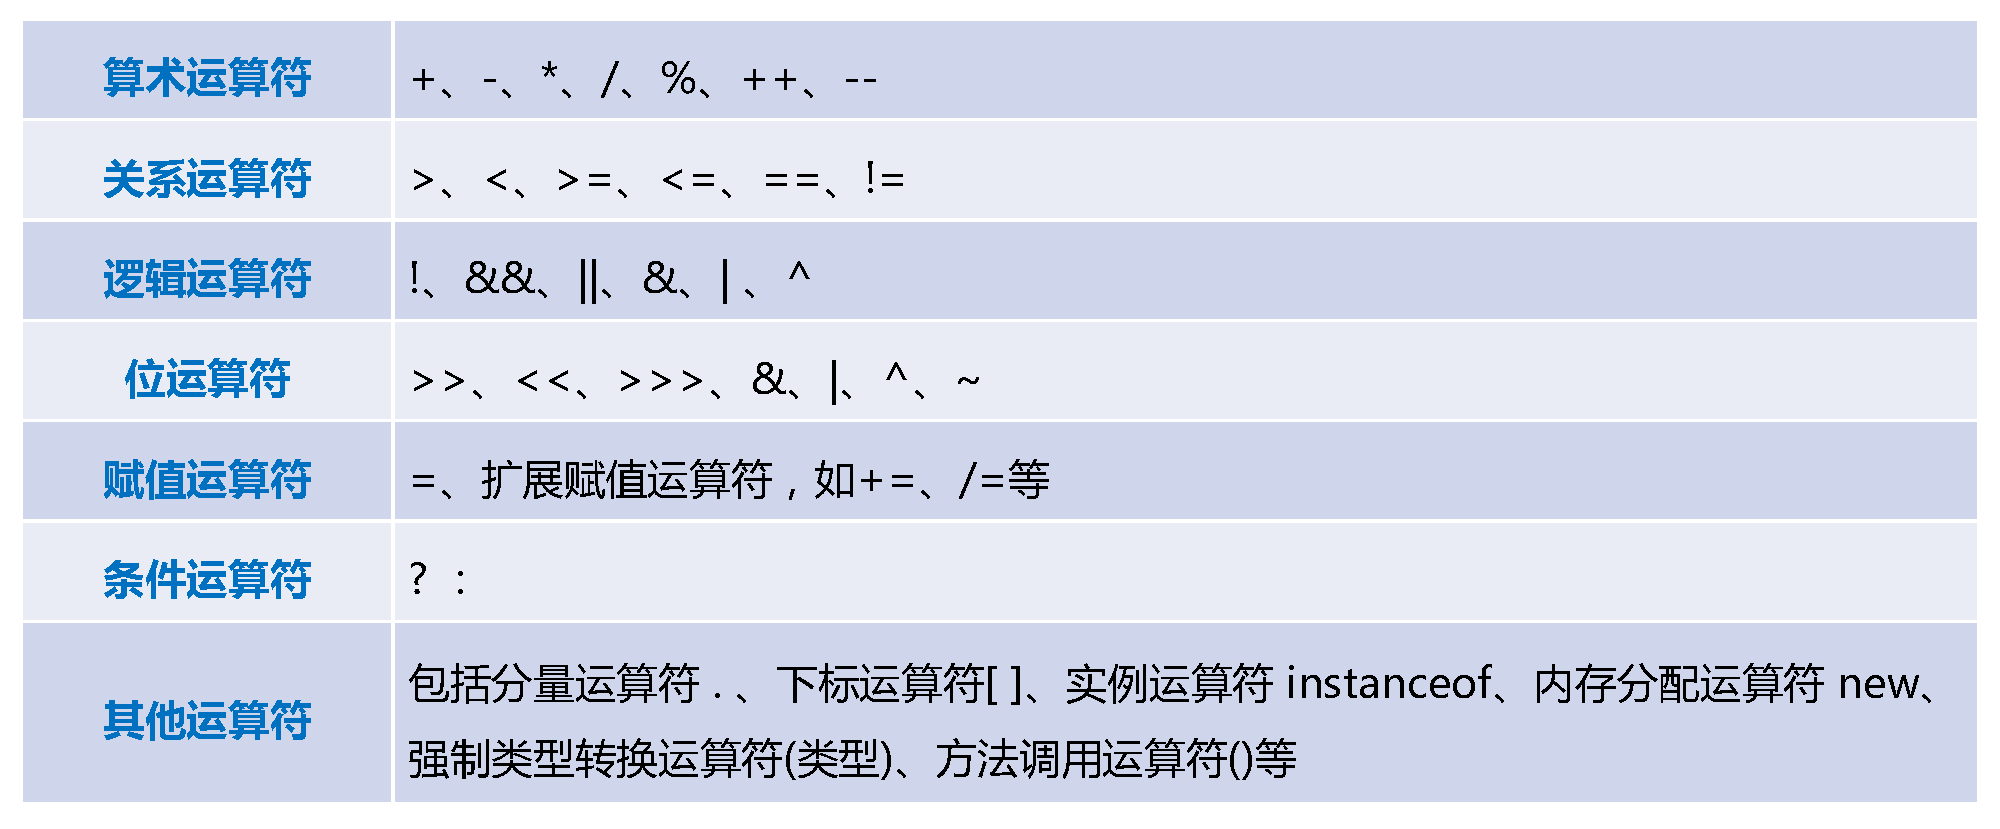
\includegraphics[width=\textwidth]{ppt/operators.pdf}
  \end{figure}

  \homework{请自行总结Java运算符的基本用法,包括运算符的优先级。}
  
\end{frame}

\section{从键盘获得输入}

\begin{frame}[fragile]
  \frametitle{从键盘获得输入}

  由键盘输入的数据,不管是文字还是数字,Java皆视为{\hei\Red 字符串},若是要由键盘输入获得数字则必须再经过类型转换。

  \samp{获得键盘输入字符串并转换为数字}

  \begin{javaCode}
    import java.io.*;
    public class MyClass {
      public static void main(String[] args) throws IOException {
        int num1, num2;
        String str1, str2;
        InputStreamReader in;
        in = new InputStreamReader(System.in);
        BufferedReader buf;
        buf = new BufferedReader(in);
        System.out.print("请输入第一个数:");
        str1 = buf.readLine();         //将输入的内容赋值给字符串变量 str1
        num1 = Integer.parseInt(str1);   //将 str1 转成 int 类型后赋给 num1
        System.out.print("请输入第二个数:");
        str2 = buf.readLine();         //将输入的内容赋值给字符串变量 str2
        num2 = Integer.parseInt(str2);   //将 str2 转成 int 类型后赋给 num2
        System.out.println(num1 + " * " + num2 + " = " + (num1 * num2));
      }
    }
  \end{javaCode}
\end{frame}

\begin{frame}[fragile]
  \frametitle{从键盘获得输入}

  为了简化输入操作,从JavaSE 5版本开始在java.util类库中新增了一个类专门
  用于输入操作的类{\bf\Red Scanner},可以使用该类输入一个对象。

  \samp{使用Scanner获得键盘输入并转换为特定数据类型}
  \begin{javaCode}
    import java.util.*;
    public class MyClass {
      public static void main(String[] args)
      {
        Scanner reader = new Scanner(System.in); 
        double num;
        num = reader.nextDouble(); //按照 double 类型读取键盘输入
        ...
      }
    }
  \end{javaCode}

  \xyy{其他可用的读取方法}
  
  {\small\Blue nextByte() nextDouble() nextFloat() nextInt() nextLong() nextShort() next() nextLine()}
\end{frame}

\section{语句}

\begin{frame}[fragile]
  \frametitle{语句与复合语句}
  \begin{itemize}
  \item Java语言中语句可以是以分号“;”结尾的简单语句,也可以是用一对花括号“\{\}”括起来的复合语句。
  \item Java中的注释形式:
    \begin{itemize}\small\Blue
    \item 单行注释://
    \item 多行注释:/*    */
    \item 文件注释:/**   */
    \end{itemize}
  \end{itemize}

\end{frame}

\section{分支结构}

\begin{frame}[fragile]
  \frametitle{分支结构}

  \wxd{if分支结构 1}
  
  \begin{figure}
    \centering
    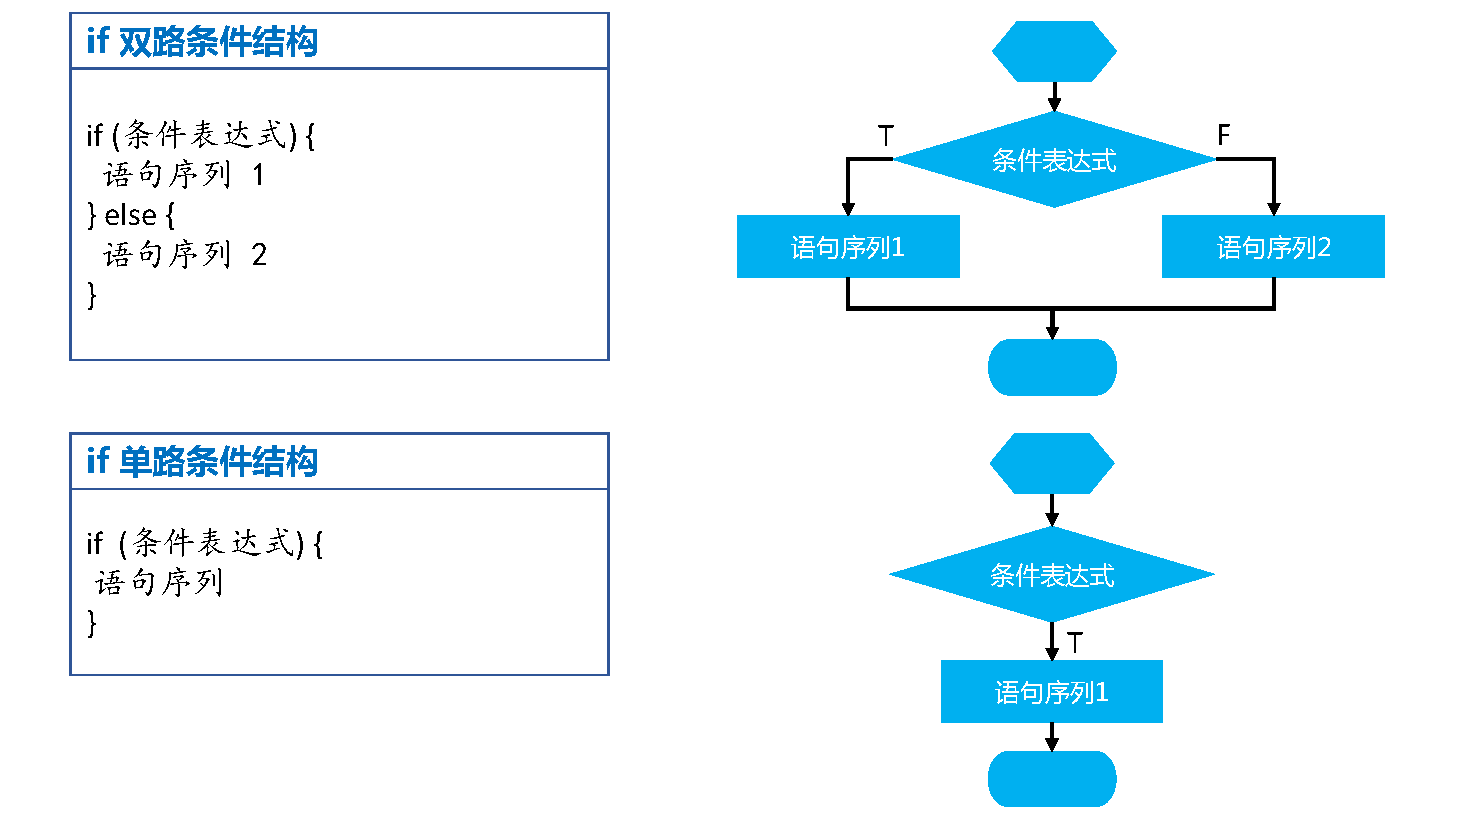
\includegraphics[width=\textwidth]{ppt/flow-control-1.pdf}
  \end{figure}

\end{frame}

\begin{frame}[fragile]
  \frametitle{分支结构}

  \wxd{if分支结构 2}
  
  \begin{figure}
    \centering
    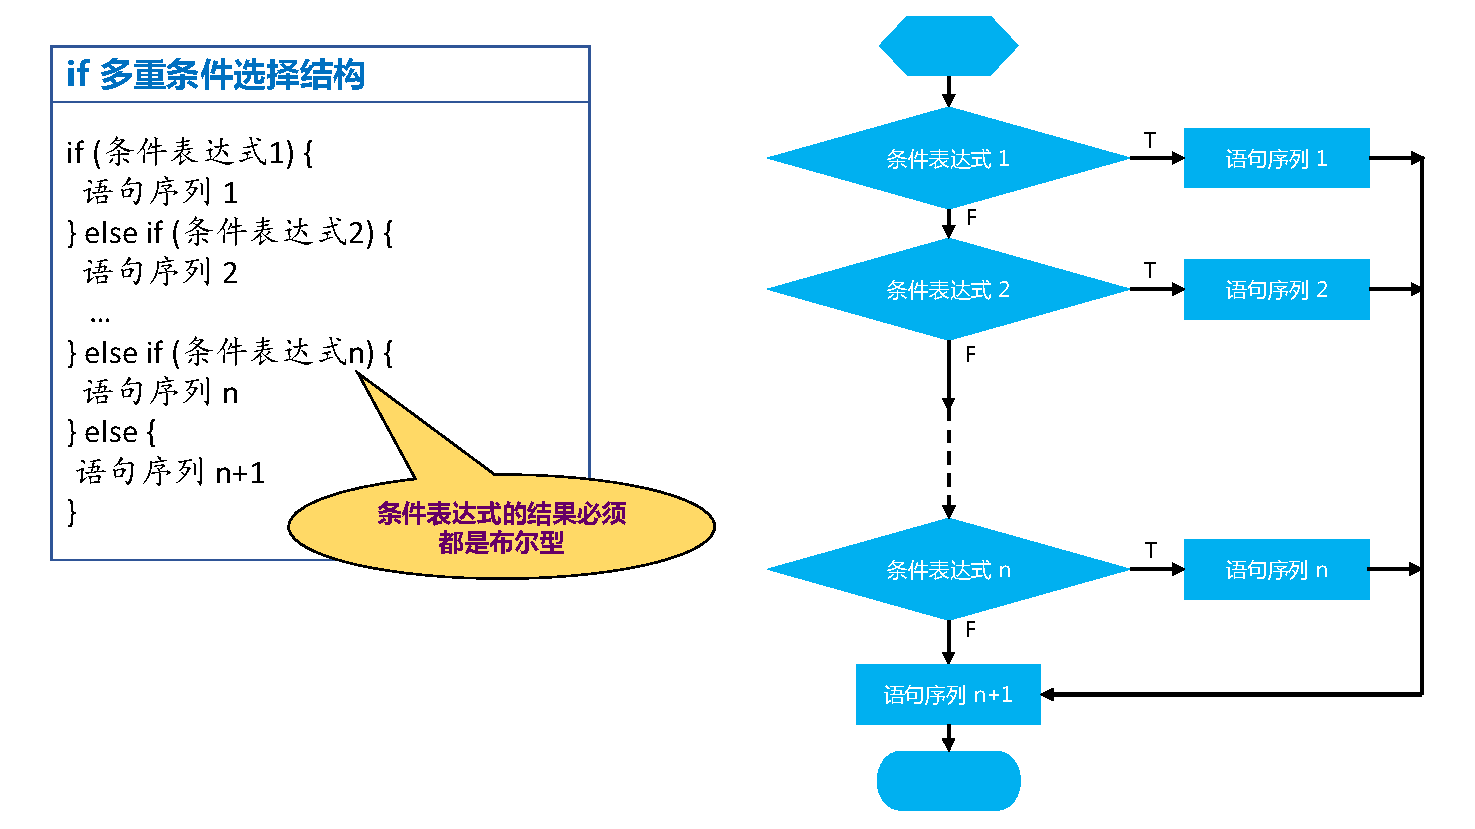
\includegraphics[width=\textwidth]{ppt/flow-control-2.pdf}
  \end{figure}

\end{frame}

\begin{frame}[fragile]
  \frametitle{分支结构}

  \wxd{switch分支结构\footnote{在Java 1.7版本之后,switch里表达式的类型可以为String。}}
  
  \begin{figure}
    \centering
    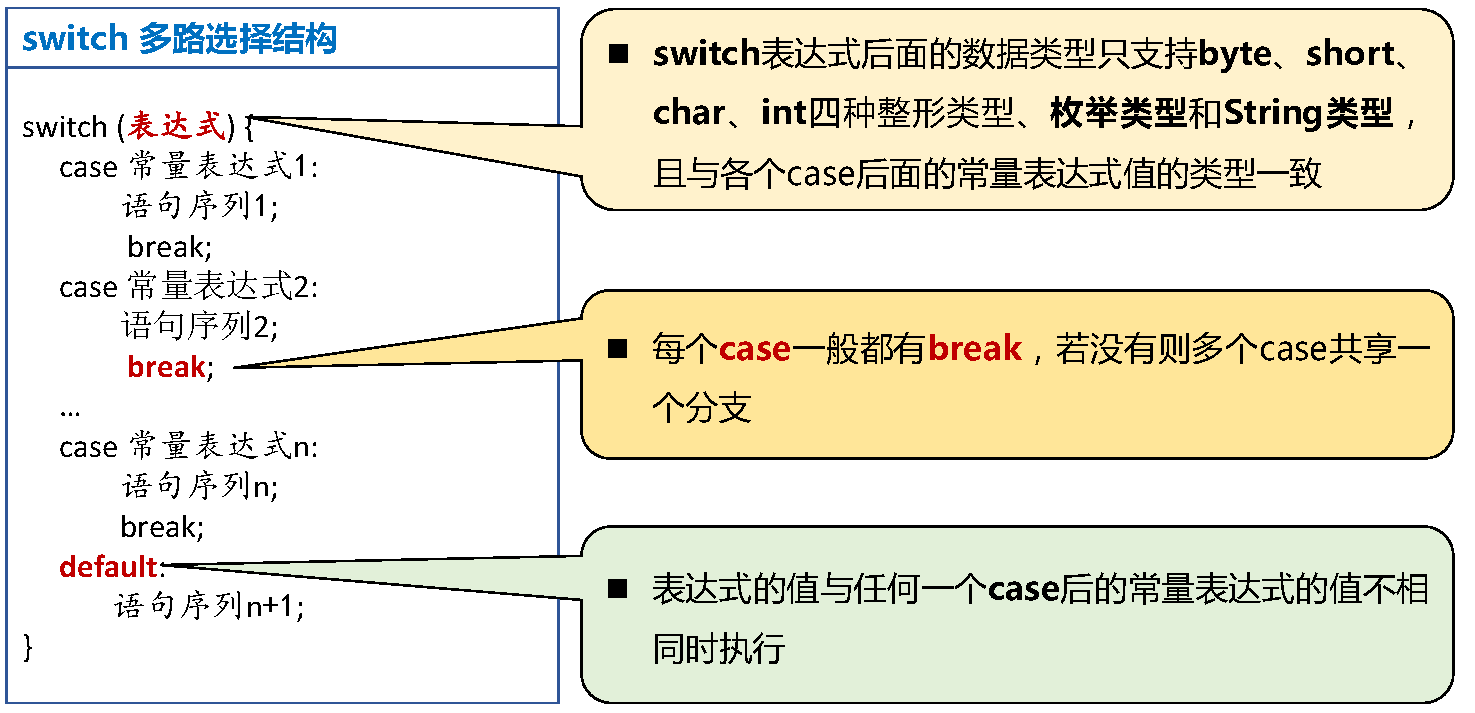
\includegraphics[width=.8\textwidth]{ppt/flow-control-3.pdf}
  \end{figure}

  \homework{自行搜索总结switch中的case语句如果没有break会出现什么情况,程序逻辑是如何执行的。}
\end{frame}

\section{循环结构}

\begin{frame}[fragile]
  \frametitle{循环结构}

  \wxd{while循环}

  \begin{javaCode}
    while(conditional expression) {
      statements goes here ...
    }
  \end{javaCode}

  \wxd{do-while循环}

  \begin{javaCode}
    do {
      statements goes here ...
    }
    while(conditional expression);
  \end{javaCode}
\end{frame}



\begin{frame}[fragile]
  \frametitle{循环结构}

  \wxd{for循环 1}

  \begin{javaCode}
    int[] integers = {1, 2, 3, 4};

    for (int j = 0; j < integers.length; j++) {
      int i = integers[j];
      System.out.println(i);
    } 
  \end{javaCode}

  \wxd{for循环 2}

  \begin{javaCode}
    int[] integers = {1, 2, 3, 4};

    for (int i : integers) {
      System.out.println(i);
    }
  \end{javaCode}
\end{frame}

\begin{frame}[fragile]
  \frametitle{循环中的跳转}
  \begin{description}\kai
  \item[break语句] 使程序的流程从一个语句块(switch或循环结构)内跳出。
  \item[continue语句] 终止当前这一轮(次)的循环,进入下一轮(次)循环。
  \item[return语句] 用来使程序从方法(函数)中返回,可返回一个值。
  \end{description}
\end{frame}

\begin{frame}
  \frametitle{本节习题}

  \wxd{简答题}
  \begin{enumerate}
  \item Java语言定义类哪些基本数据类型?其存储结构分别是什么样的?
  \item 自动类型转换的前提是什么?转换时的优先级顺序如何?
  \item 数字字符串转换为数值类型数据时,可以使用的方法有哪些?
  \end{enumerate}

  \wxd{小编程}
  \begin{enumerate}
  \item 编写程序,从键盘输入一个浮点数,然后将该浮点数的整数部分输出。
  \item 编写程序,从键盘输入2个整数,然后计算它们相除后得到的结果并输出,注意排除0除问题。
  \end{enumerate}
\end{frame}

%%%%%%%%%%%%%%%%%%%%%%%%%%%%%%%%%%%%%%%%%%%%%%%%%%%%%%%%%%%%%%%%%%%%%%%%%%%%%%%
% TKS Page %%%%%%%%%%%%%%%%%%%%%%%%%%%%%%%%%%%%%%%%%%%%
\begin{frame}
\centering
{\Huge \textcolor{blue}{THE END}} \\
\vspace{5mm}
{\Large wangxiaodong@ouc.edu.cn} \\
\end{frame}
%%%%%%%%%%%%%%%%%%%%%%%%%%%%%%%%%%%%%%%%%%%%%%%%%%%%%%%
%%%%%%%%%%%%%%%%%%%%%%%%%%%%%%%%%%%%%%%%%%%%%%%%%%%%%%%%%%%%%%%%%%%%%%%%%%%%%%%
\end{document}
